\noindent

\begin{figure}[t!]
  \begin{center}
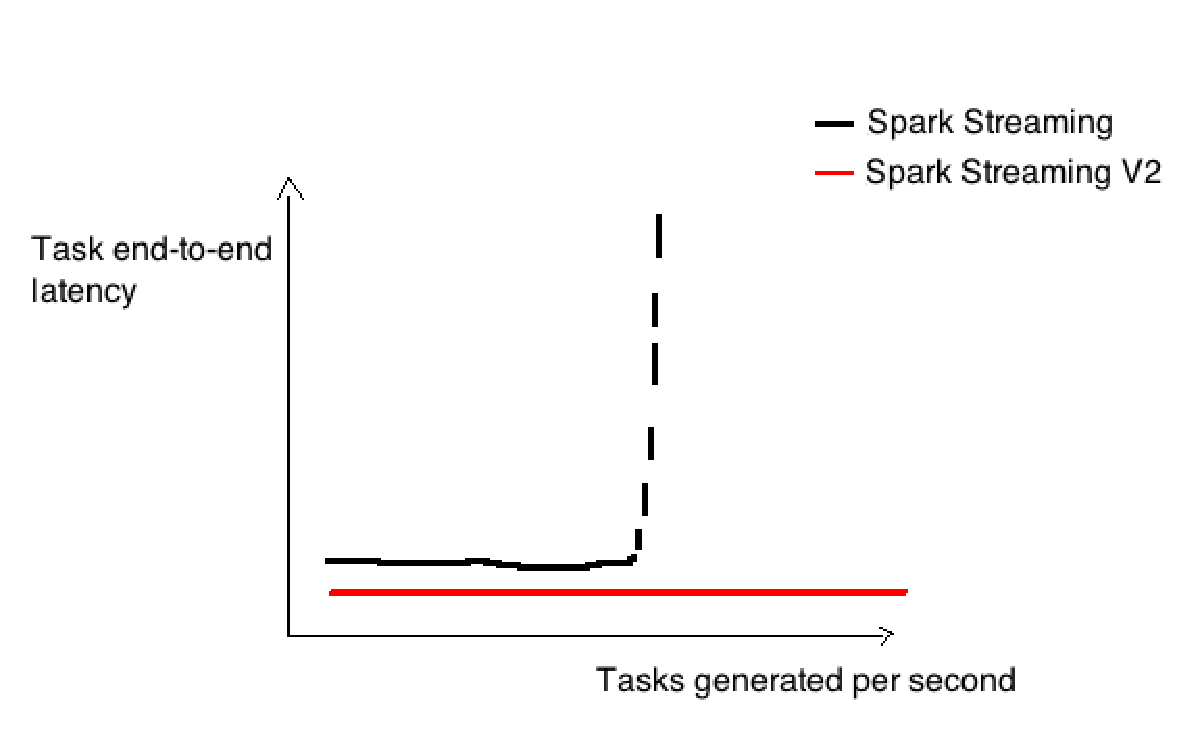
\includegraphics[scale=0.4]{money_graph.eps}
  \end{center}
  \caption{End-to-end latency of individual tasks for varying task generation rates. Improvement results of our proposed techniques.}
  \label{fig:money_graph}
\end{figure}

This paper tries to present a solution for stream processing of short tasks in Spark Streaming - a space that we have found Spark Streaming lacking in practice.
We present three techniques to achieve this goal: 1) reduction of task overheads, 2) decentralized and elastic scheduling, and 3) leveraging modern network mediums of communication for faster transfer of data between the driver, schedulers and workers.

Much of this work is still in progress. We plan to continue working on this problem and evaluating the solutions we have proposed. Figure~\ref{fig:money_graph} shows the result we want to obtain with the techniques we have proposed. We expect the average end-to-end latency of tasks to be lower and the scheduling "capacity" to be higher and a function of the available hardware resources.
